\chapter{Development and Setup of Experiments}
\section{Initial Development}
In order to determine the possibilities and limitations of making observations with a compact spectrograph similar to the USB4000, it was necessary to preform initial testing on the USB4000. 
To examine the spectrograph it was decided to develop different setups to test the stability of the measurements. In an orbit in space the spectrograph will be pointed at different astronomical objects to analyze the light they radiate and thereby analyze the properties of the objects. 

In the laboratory, however, the light source observed by the spectrograph was chosen to be a light source with a very well known spectrum in the wavelength range of the spectrograph. For a well known light source and its spectrum, the laboratory wavelength, which is the wavelength measured in vacuum, of an emission line located in the spectrum is well documented, which enables the spectrograph to be calibrated.  
Upon the development of the setups it was necessary to consider what kind of environment the spectrograph could be subject to if it was launch to space. 

% NOget med MONS satelitte

As mentioned in section \ref{satellite}, the two main common factors for a spacecraft in orbit, are movement due to pointing of the spacecraft and variations of the temperature inside the spacecraft. Furthermore the observations of astronomical objects are often performed over a long duration of time, which means measurements taken over a long period of time must be stable. With these factors taken in to consideration, three experiment setups with different purposes were designed,

\begin{enumerate}
\item Stationary Experiment - Analysis of measurements with the spectrograph being stationary.
\item Simulated Pointing Experiment - Analysis of measurements with the spectrograph with simulation of pointing via vibrations.
\item Temperature Dependence Experiment - Analysis of measurements with the spectrograph at different temperatures.
\end{enumerate}



The development, purpose and improvements of the three experiments and the calibration of the spectrograph will be discussed in the following sections.

\subsection{Calibration of the USB4000 Spectrograph}
The relationship between pixel number and wavelength for the USB4000 is given by a third-order polynomial,\footnote{\url{http://oceanoptics.com/product/usb4000-custom/}}
\begin{equation}
 \lambda _p = I +C_1p + C_2 p^2 + C_3 p^3  ,
 \label{eq: calib}
\end{equation}
where $\lambda_p$ is the wavelength of the pixel \emph{p}, $I$ is the wavelength of pixel 0, and $C_1,C_2,C_3$ are the coefficients of the equation. By using a well known light spectrum with documented spectral emission lines the pixels of the CCD can be calibrated. With the Helium calibration lamp described below, this was done for the USB4000 by taking a measurement of the spectrum from the calibration lamp. The known wavelengths for the spectral emission lines of the lamp, shown in Tbl. \ref{tbl: Helium peaks}, were then fitted to Eq. \ref{eq: calib} with the pixel numbers for the measured lines. The calibration values calculated for the USB4000 are shown in Tbl. \ref{tbl: calib}.

\begin{table}[h]
\centering
    \begin{tabular}{cccc}
    \hline
    $I$ [nm]& $C_1$ [$\frac{nm}{pixel}$]& $C_2$ [$\frac{nm}{pixel^2}$]& $C_3$[$\frac{nm}{pixel^3}$] \\ \hline
    ~
    177.47  & \num{2.2140d-5}    & \num{-6.1407d-6}    & \num{-2.8831d-10}    \\ \hline
    \end{tabular}
    \caption{Calibration values for the USB4000.}
    \label{tbl: calib}
\end{table}

\subsection{Helium Spectrum}
\label{sec: Helium}
To examine the stability of the spectrograph, six spectral emission lines within the Helium spectrum were used. Helium has well known spectral emission lines that are well defined and distributed across the wavelength range of the spectrograph. The use of well defined spectral emission lines ensures that any broadening or shift of the spectral lines are detectable. In Fig. \ref{fig: Helium spectrum} the spectral emission lines in the Helium spectrum in the range 380-900 nm are shown.

\begin{figure}[h!]
\centering
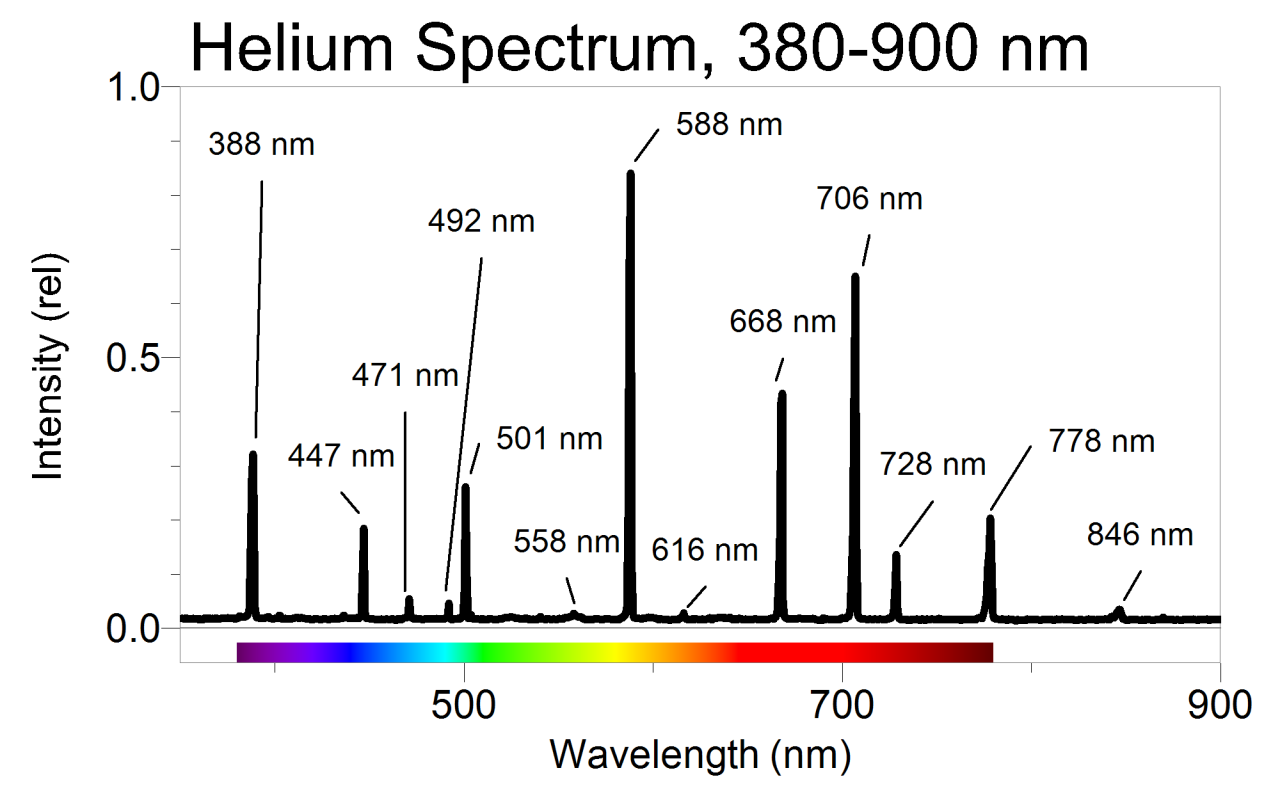
\includegraphics[width = \linewidth]{Helium_spectrum.png}
\caption[]{Spectral lines in the Helium spectrum in the range \SIrange{380}{900}{\nano\m}. Fig. from \citep{helium}.}
\label{fig: Helium spectrum}
\end{figure}



\section{First Experiment- Stationary Measurements}
The purpose of the first setup was to determine the stability of multiple readings over a long period of time from the spectrograph. The parts used for the first initial setup were:

\begin{itemize}
\item HeNe laser
\item  USB4000 Spectrograph with the data acquisition software, \emph{SpectraSuite}\footnote{\url{http://oceanoptics.com/wp-content/uploads/SpectraSuite.pdf}}.
\item Optical bench for mounting the setup
\end{itemize}

The HeNe laser was chosen as the first light source because it had a well documented single peak in its spectrum. The initial setup for the first experiment, is shown in Fig. \ref{fig: First setups}, where a sketch of the setup is illustrated as well as a picture of the actual setup.

\begin{figure}[ht]
\centering
\begin{subfigure}{0.65\linewidth}
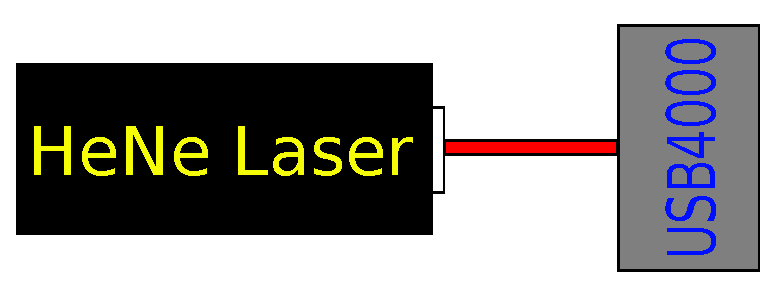
\includegraphics[width=\textwidth]{First_sketch.pdf}
\caption{Sketch of the setup for the first experiment.}
\label{fig: First_sketch}
\end{subfigure}

\begin{subfigure}{0.65\textwidth}
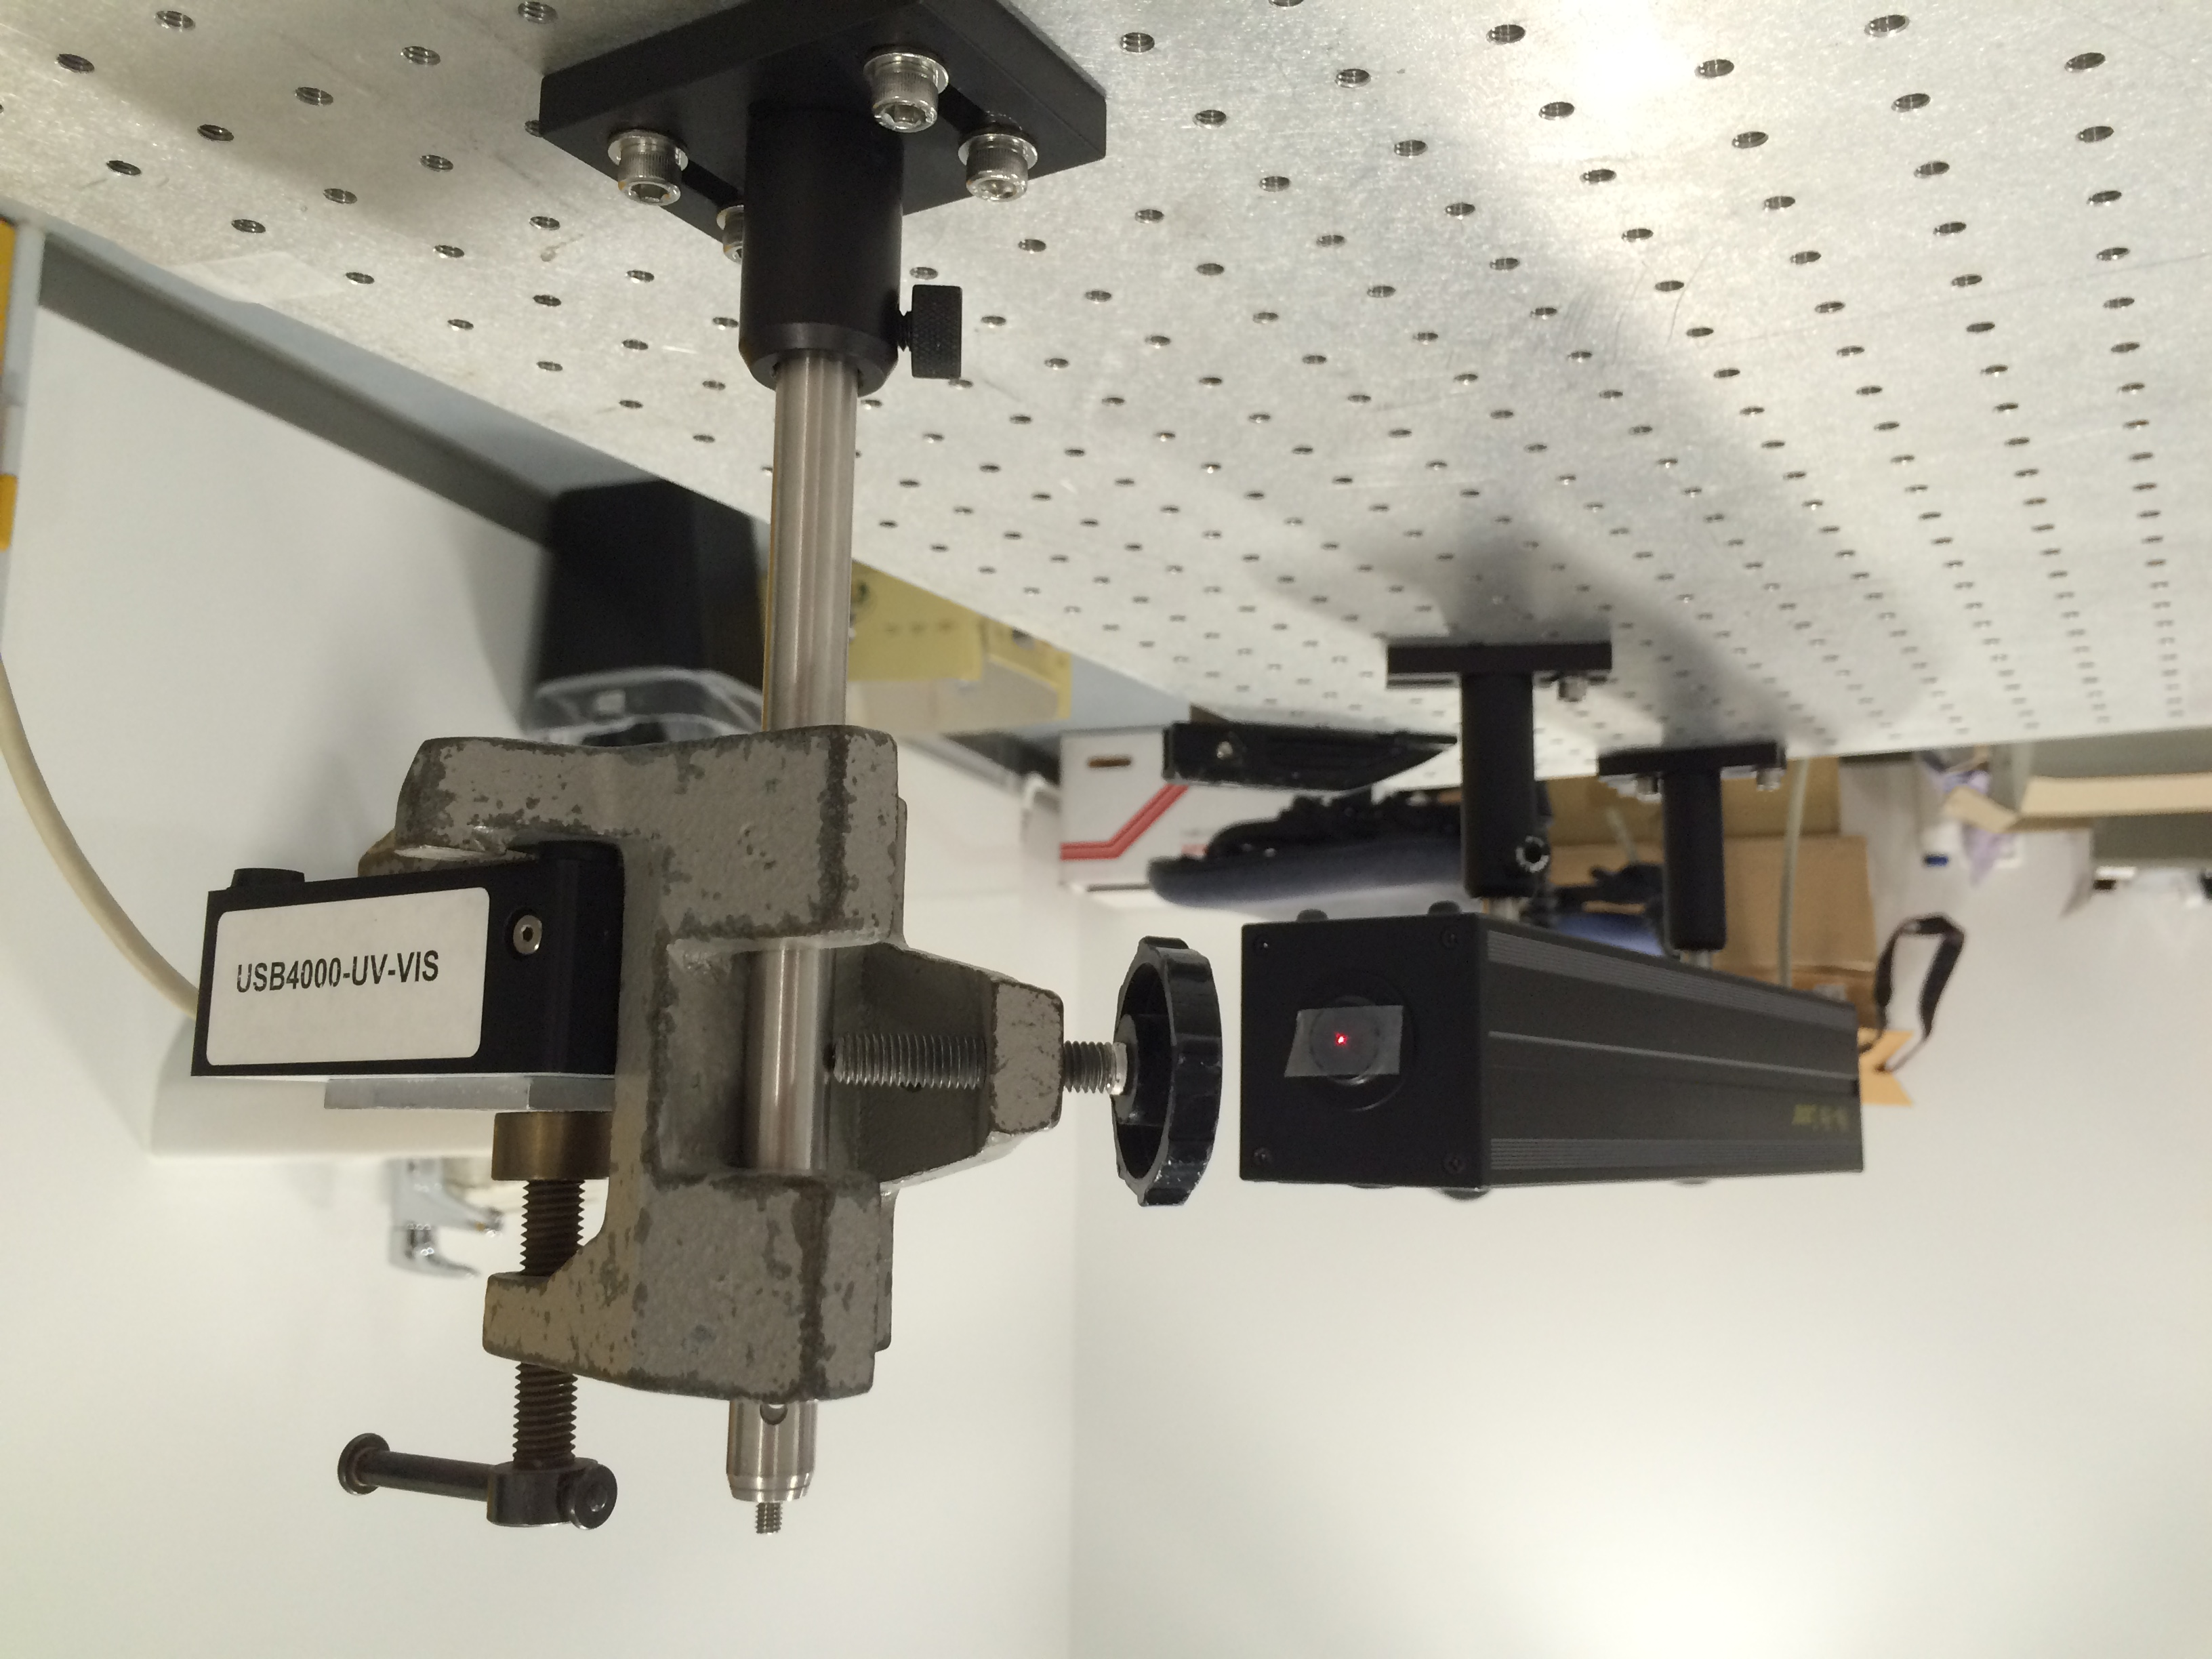
\includegraphics[width=\textwidth]{first_HeNe.JPG}
\caption{Actual setup for the first experiment.}
\label{fig: first_HeNe}
\end{subfigure}
\caption{The setup for the initial run of the stationary measurement with a HeNe laser as the light source. In the top panel a sketch of the top view of the setup is illustrated and in the bottom panel the actual setup is shown from an angle. The tape used as a scrambler is visible over the output lens of the laser.}
\label{fig: First setups}
\end{figure}

The setup for the stationary measurement was very simple as there were no moving parts or control of temperature as was done in later tests. For the execution of the experiment the HeNe laser was aligned so the light beam hit the slit of the spectrograph, which was connected to the data acquisition software, \emph{SpectraSuite}. The laser was fitted with tape across the output lens, this was done because the tape performs like a scrambler which causes the light beam to become more uniform. This was done as an attempt to make the setup less sensitive to alignment of the laser beam on to the spectrograph slit. The parameters for the initial test were,

\begin{itemize}
\item The HeNe Laser was set to an output of \SI{1}{\milli\watt} and the tape was used as a scrambler by placing it over the exit slit of the laser which was pointed onto the entrance slit of the USB4000.
\item In \emph{SpectraSuite} the integration time was set to \SI{10}{\milli\second}, allowing for a high peak to be located at the expected wavelength. Measurements were done every \SI{20}{\second} for a total of \num{1000} measurements.
\item \emph{SpectraSuite} saved the intensity as a function of wavelength to a text file. No filtering of noise from the CCD or smoothing was applied.
\end{itemize}

After the run of the initial setup some problems were found,

\begin{itemize}
\item The results were dependent on the alignment of the laser and the spectrograph. Small vibrations could cause observable changes in the alignment, which caused the laser to saturate the CCD detector, making the measurements useless. 
\item The change in alignment was also able to change the form of the emission line in the measured spectrum to a very flat and wide peak, which was most likely because of internal reflections within the spectrograph.
\item Although the HeNe laser produces a well defined peak, it would be preferable if several peaks located over the range of the spectrograph could be observed, to obtain more data for analysis.
\end{itemize} 

After running the initial setup where the problems mentioned earlier were present, improvements to the setups were introduced. Most of the issues were in someway related to the use of the HeNe laser as the light source. The size of the light spot from the laser was to small compared to the entrance slit of the spectrograph, this meant that the light over the whole entrance slit was not as uniform as desired. In space, movement due to pointing, of the light hitting the slit is expected, but the intensity is not expected to be high enough to saturated the CCD.
\\
\\
For the reasons explained above for the initial setup, the light source used for measurements was changed to a Helium calibration lamp which was used for wavelength calibration as well. In this case several peaks across the measurable range could be selected in the output spectrum to observe for the experiments and the light hitting the entrance slit would be more uniformly spread out due to the lamp no focusing the light on to a small area. Furthermore the mounting to the optical bench was changed in such way that it could be used for the second test as well, which examined the instability of pointing in space via vibrations of the spectrograph. The spectrograph was therefore mounted on top of the shaft of a stepper motor. The stepper motor was mounted with four \SI{90}{\degree} angle pieces onto the optical bench next to the electronics controlling it. The stepper motor was turned off for the stationary test but could be made to move when needed in the second experiment. A sketch and the real setup can be seen in Fig. \ref{fig: setup_vib_final}.

\begin{figure}[h!]
\centering
\begin{subfigure}{0.8\textwidth}
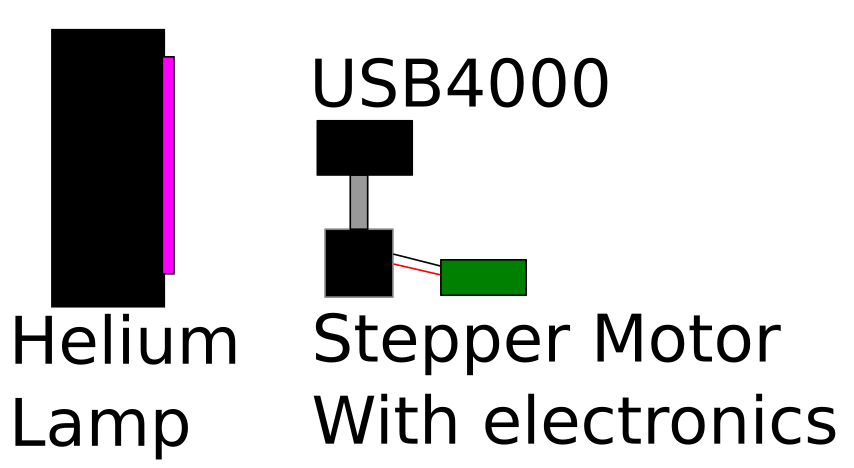
\includegraphics[width=\textwidth]{sketch_vib.png}
\caption{Sketch of setup.}
\label{fig: Vib_sketch}
\end{subfigure}

\begin{subfigure}{0.8\textwidth}
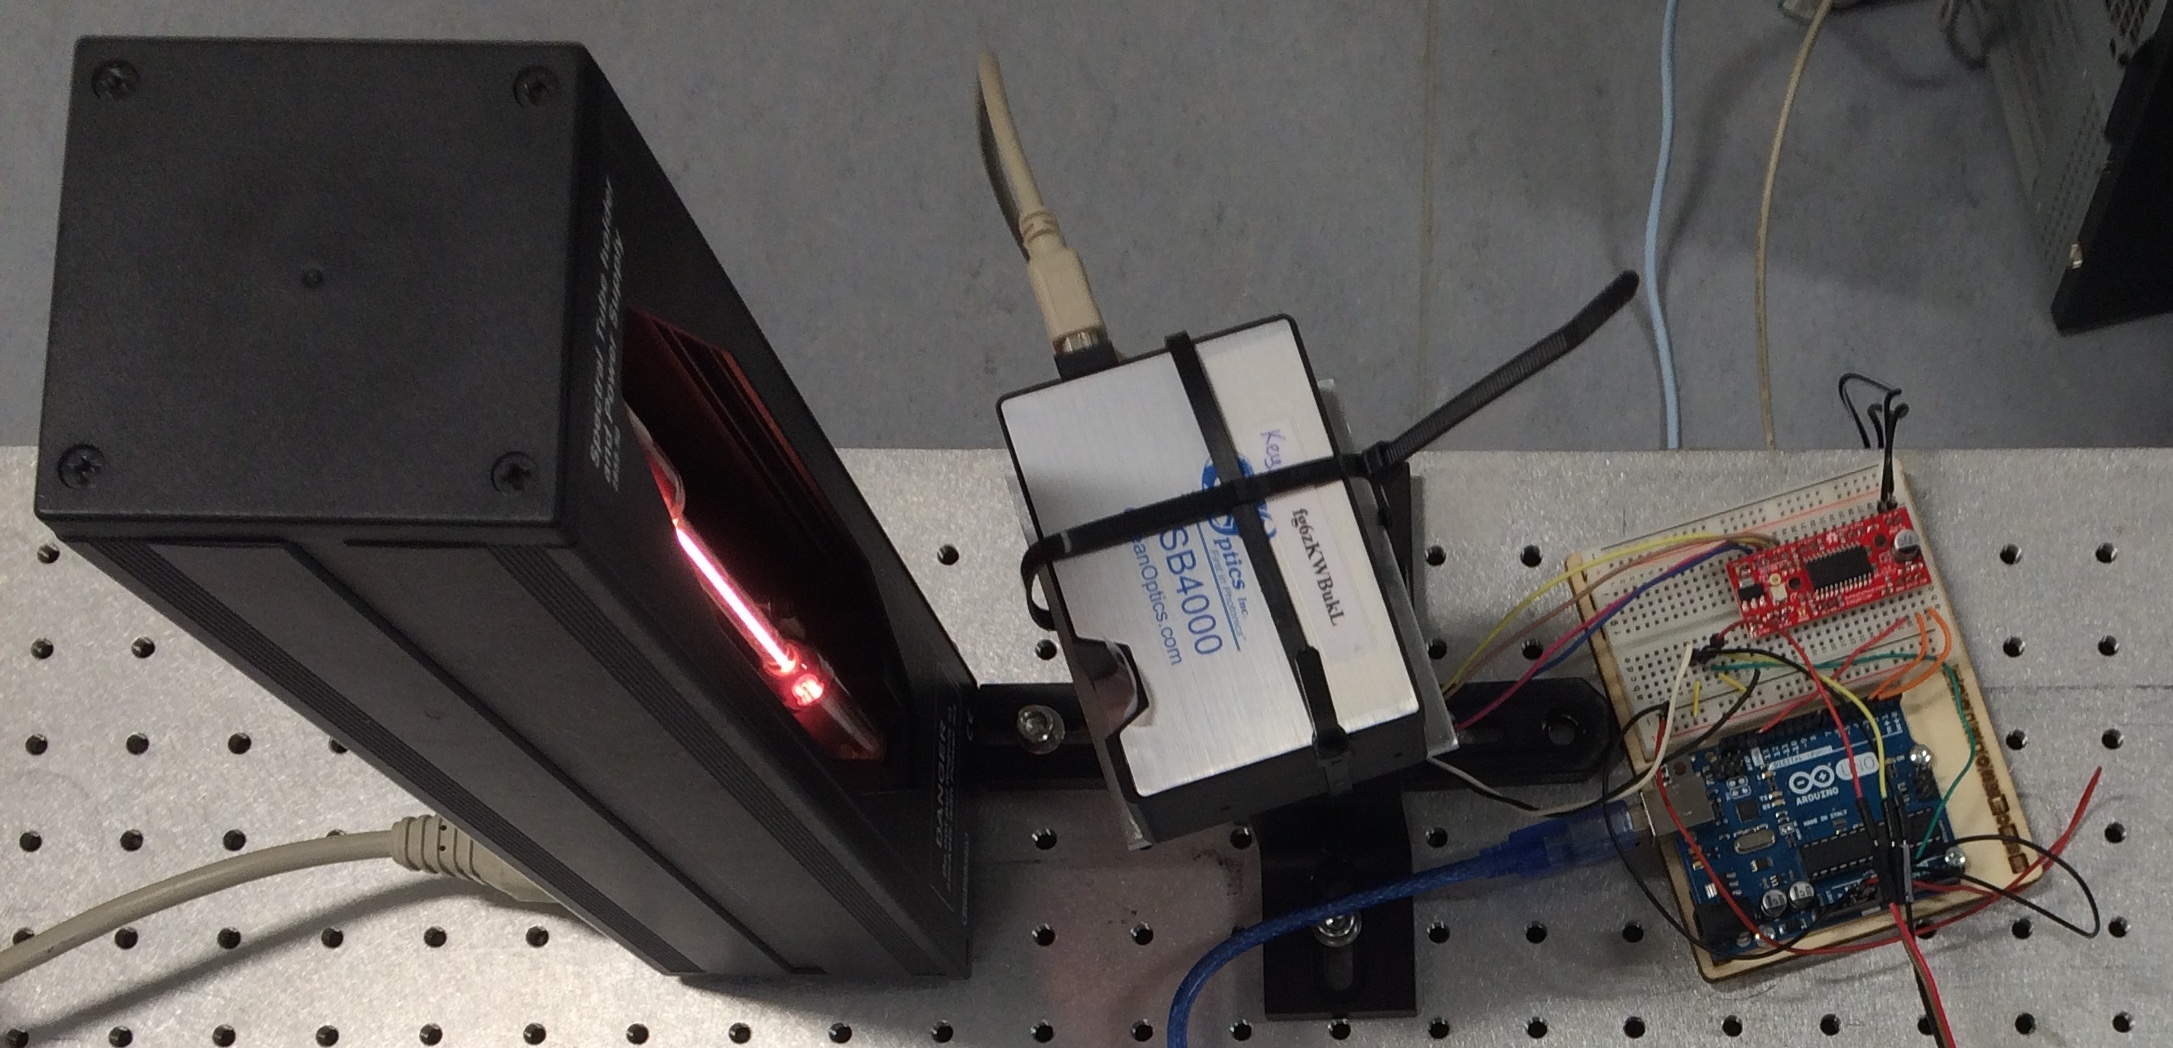
\includegraphics[width=\textwidth]{setup_vib.JPG}
\caption{Actual setup.}
\label{fig: Vib_setup}
\end{subfigure}
\caption{The final setup for both the stationary experiment and simulated pointing experiment. The top panel shows a sketch of the setup seen from the side and the bottom panel shows the actual setup. The electronics were only used to control the stepper motor in the simulated pointing experiment.}
\label{fig: setup_vib_final}
\end{figure}

The change of light source meant that the final parameters of the test were changed,
\begin{itemize}
\item The light source was changed to the Helium calibration lamp. 
\item The tape used as a scrambler was moved to the entrance slit of the spectrograph and the Helium calibration lamp was placed such that the CCD detector in the spectrograph was not saturated.
\item Integration time in \emph{Spectrasuite} was set to \SI{100}{\milli\second}. Measurements were still done every \SI{20}{\second} for a total of \num{1000} measurements, and saved to a text file with the intensity for every wavelength for data processing.
\end{itemize}

\section{Second Experiment - Simulated Pointing}
The purpose of the second experiment was to test the stability of the measurements from the spectrograph, when it was exposed to vibrations, to simulate pointing of the satellite. The setup for the second experiment included the parts used for the final setup in the stationary experiment in addition to,
\begin{itemize}
\item The stepper motor was now used to simulate the pointing of the spacecraft by rotating the spectrograph back and forth over an angle spanning \SI{45}{\degree}. The rotation was done with a frequency of \SI{1.04}{\Hz}, which allowed for enough light exposure at the different angles for the spectrograph to obtain detectable peaks in the output spectrum. 
\item The electronics used to control the stepper motor were the two commercial development boards, \emph{Raspberry Pi} and \emph{Arduino Uno}. These were programmed to moved the stepper motor at the desired frequency.
\item Measurements were taken every \SI{20}{\second} for a total of a \num{1000} measurements. Every measurement was saved to a text file, with the intensity as a function of wavelength.
\end{itemize}

The setup was the same as for the stationary measurement which can be seen in Fig. \ref{fig: setup_vib_final}.

\section{Third Experiment - Temperature Dependence}
The purpose of the third experiment was to determine the temperature dependency of the measurements from the spectrograph. For this experiment it was necessary to build a housing environment were  the temperature could be controlled as precisely as possible. The system would need to be well insulated so the temperature inside could be kept stable for long enough time to allow the temperature of the spectrograph to come in to equilibrium with the set temperature. In orbit the temperature will vary from \SI{-10}{\degreeCelsius} to \SI{40}{\degreeCelsius} on a 90 minute cycle. Because the housing of the spectrograph was not opened the temperature inside can not be measured directly, this is why each temperature is hold for long duration to ensure that the spectrograph is at the set temperature of the housing. Furthermore a window for the light to enter the housing was preferable as this would allow the light source to be placed outside the housing, allowing for a smaller volume in which the temperature needed to be controlled. For the actual heating of the housing and how to control the temperature precisely, different methods were considered,

\begin{itemize}
\item A hot air blower manually set to different temperatures.
\item Thermoelectric cooling by using a Peltier device, which can transfer heat from one side of the device to the other depending on the direction of the current going through it, thereby being able to heat up one of the device sides. 
\item A heater circuit design by ourselves and controlled by a PID temperature controller.
\end{itemize}

For the use of a hot air blower  the housing for the experiment would quickly become complicated to build, to allow for a hot air entrance without a large heat loss, which could cause the temperature to be unstable. A Peltier device is mainly used for cooling purposes by ensuring that the hot side of the device itself is cooled. Thereby allowing the cold side to be cooled even further by transferring its excess heat to the hot side. It would be to time consuming  to develop a setup that worked with precision control of the hot side of the Peltier device. 
\\
\\
Therefore we used a setup using a heater circuit we designed ourselves, that could keep the volume of the housing small and would only need a few wires to be run inside the housing. The heater circuit was controlled by an \emph{Arduino Uno} running PID controller software.
After discussing with the electronics department of Aarhus University Institute for Physics and Astronomy, a simple circuit was designed which satisfied our needs. The circuit schematics can be seen in Fig. \ref{fig: circuit}. The circuit is run of a \SI{12}{\volt} power supply, with the positive terminal connected to a power resistor, functioning as the heating element of the circuit. The high power resistor is capable of having large amounts of power delivered to it, causing it to heat up as current flows through it and as the voltage drops across it. The resistor was connected to ground through a transistor controlled by the \emph{Arduino Uno}. The transistor works as a switch, which connects the collector and emitter legs of the transistor when a voltage is applied to the base leg. The resistor was connected to the collector leg and the emitter leg was connected to ground, while the base leg was connected to the \emph{Arduino Uno} with the PID software. The PID software  controlled when and for how long the collector and emitter legs were connected based on the temperature readings from a temperature sensor connected to the \emph{Arduino Uno} from inside the test housing. With the wanted temperature inside the housing being adjustable from the PID software, the experiment could be run without the need to physical interrupt the setup. 
\\
\\
After deciding on a wanted design, an initial test setup was build to ensure the heating circuit and PID controller were working as planned. The setup was constructed with the following parts:
\begin{itemize}
\item The housing was made from a small cardboard box, as high insulation was not needed for testing if the heater circuit and PID controller worked as expected. This setup is shown in Fig. \ref{fig: cardboard}.
\item A 12 V power supply, BD649 Transistor, SH650 Resistor and TMP35 Temperature sensor.\footnote{Component Data sheets : \url{http://www.alldatasheet.com}}
\end{itemize}

\begin{figure}[h]
\centering
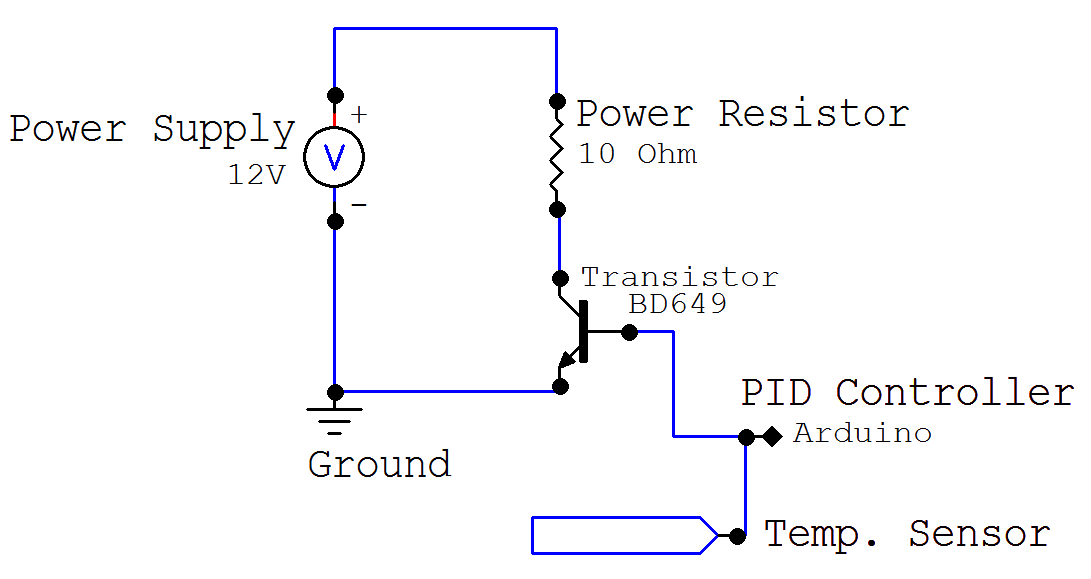
\includegraphics[width =\linewidth]{kredslob.png}
\caption{Schematic view of the heater circuit used to control the temperature in the housing for the temperature dependence experiment.}
\label{fig: circuit}
\end{figure}

The spectrograph was placed in the housing with a window for the light to enter. Tape was used to insulate the window and works as a scrambler like in the previous experiments. The power resistor was mounted on a heatsink in contact with the spectrograph, the temperature sensor was mounted on the spectrograph as well. The power resistor and temperature sensor were mounted directly onto the spectrograph because it was expected to provide the fastest heating and most stable temperature readings. A small fan was put in the housing to circulate the air to get a uniform temperature inside the housing. The cables were then run outside the housing to the remaining circuit. The setup inside and outside the housing is shown in Fig. \ref{fig: cardboard}.

\begin{figure}[h!]
\centering
\begin{subfigure}{.5\textwidth}
\centering
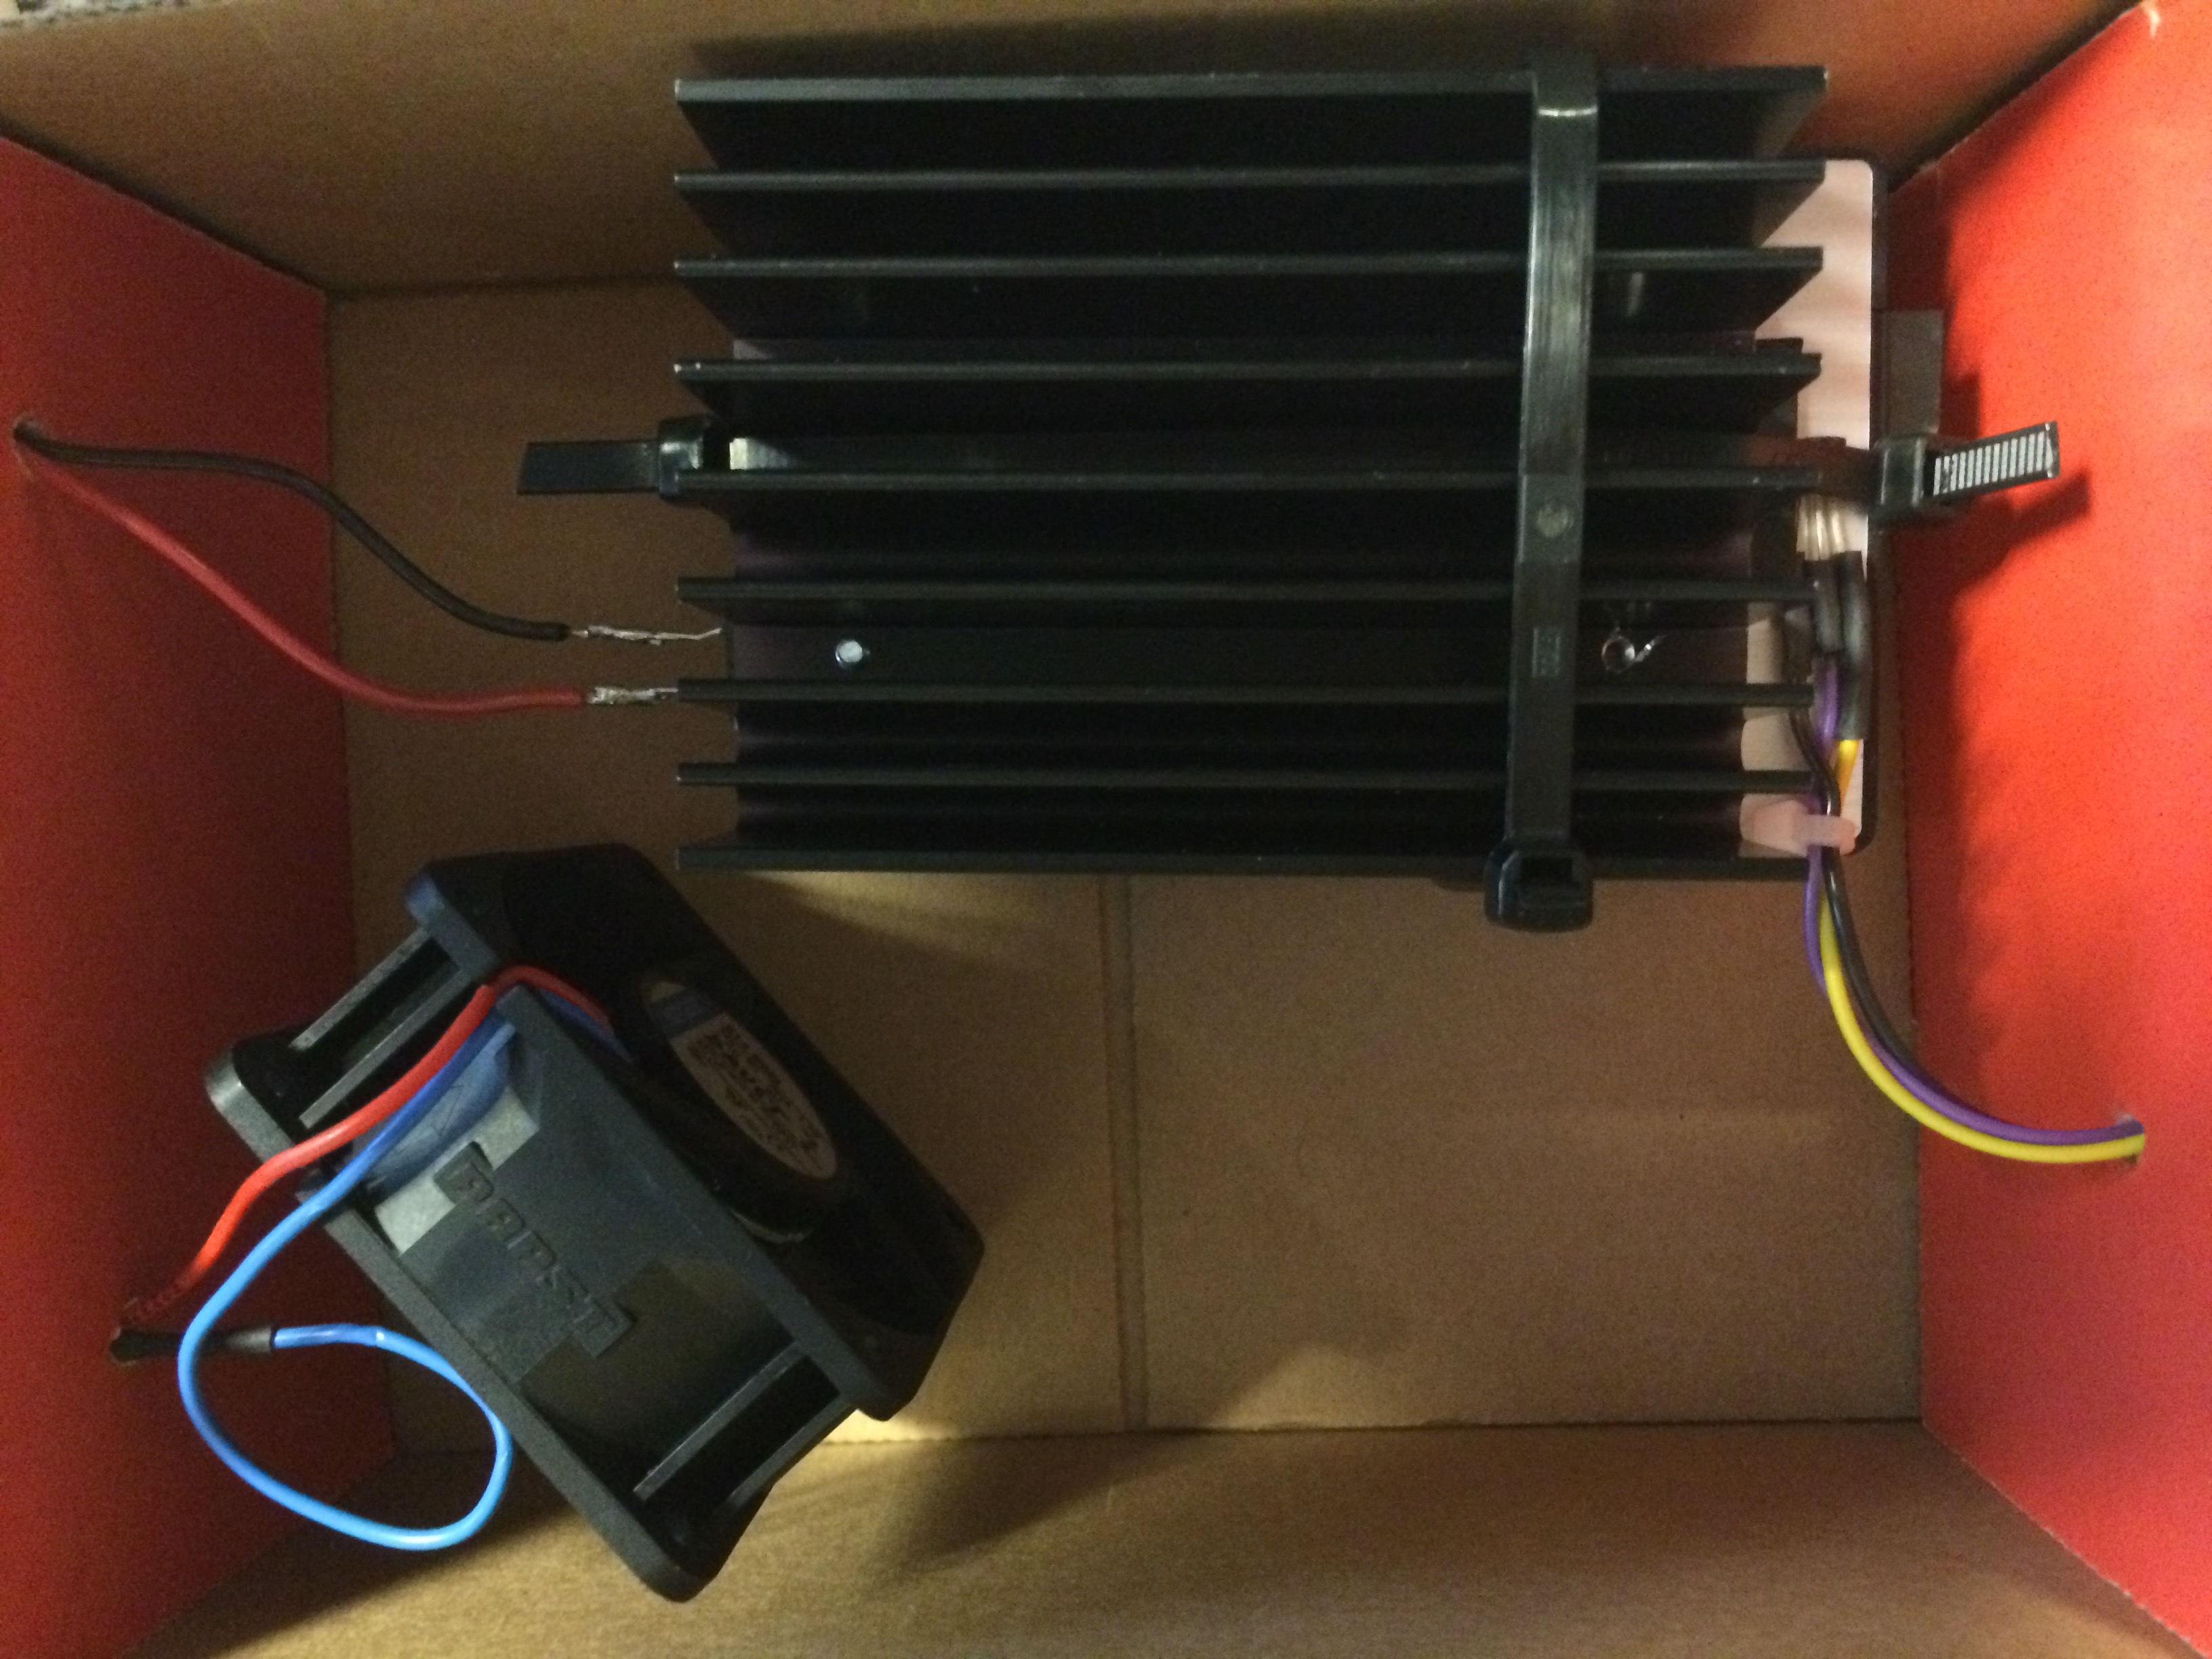
\includegraphics[width=.95\linewidth]{cb_circuit.JPG}
\caption{Inside of housing.}
\label{fig: cd_circuit}
\end{subfigure}%
\begin{subfigure}{.5\textwidth}
\centering
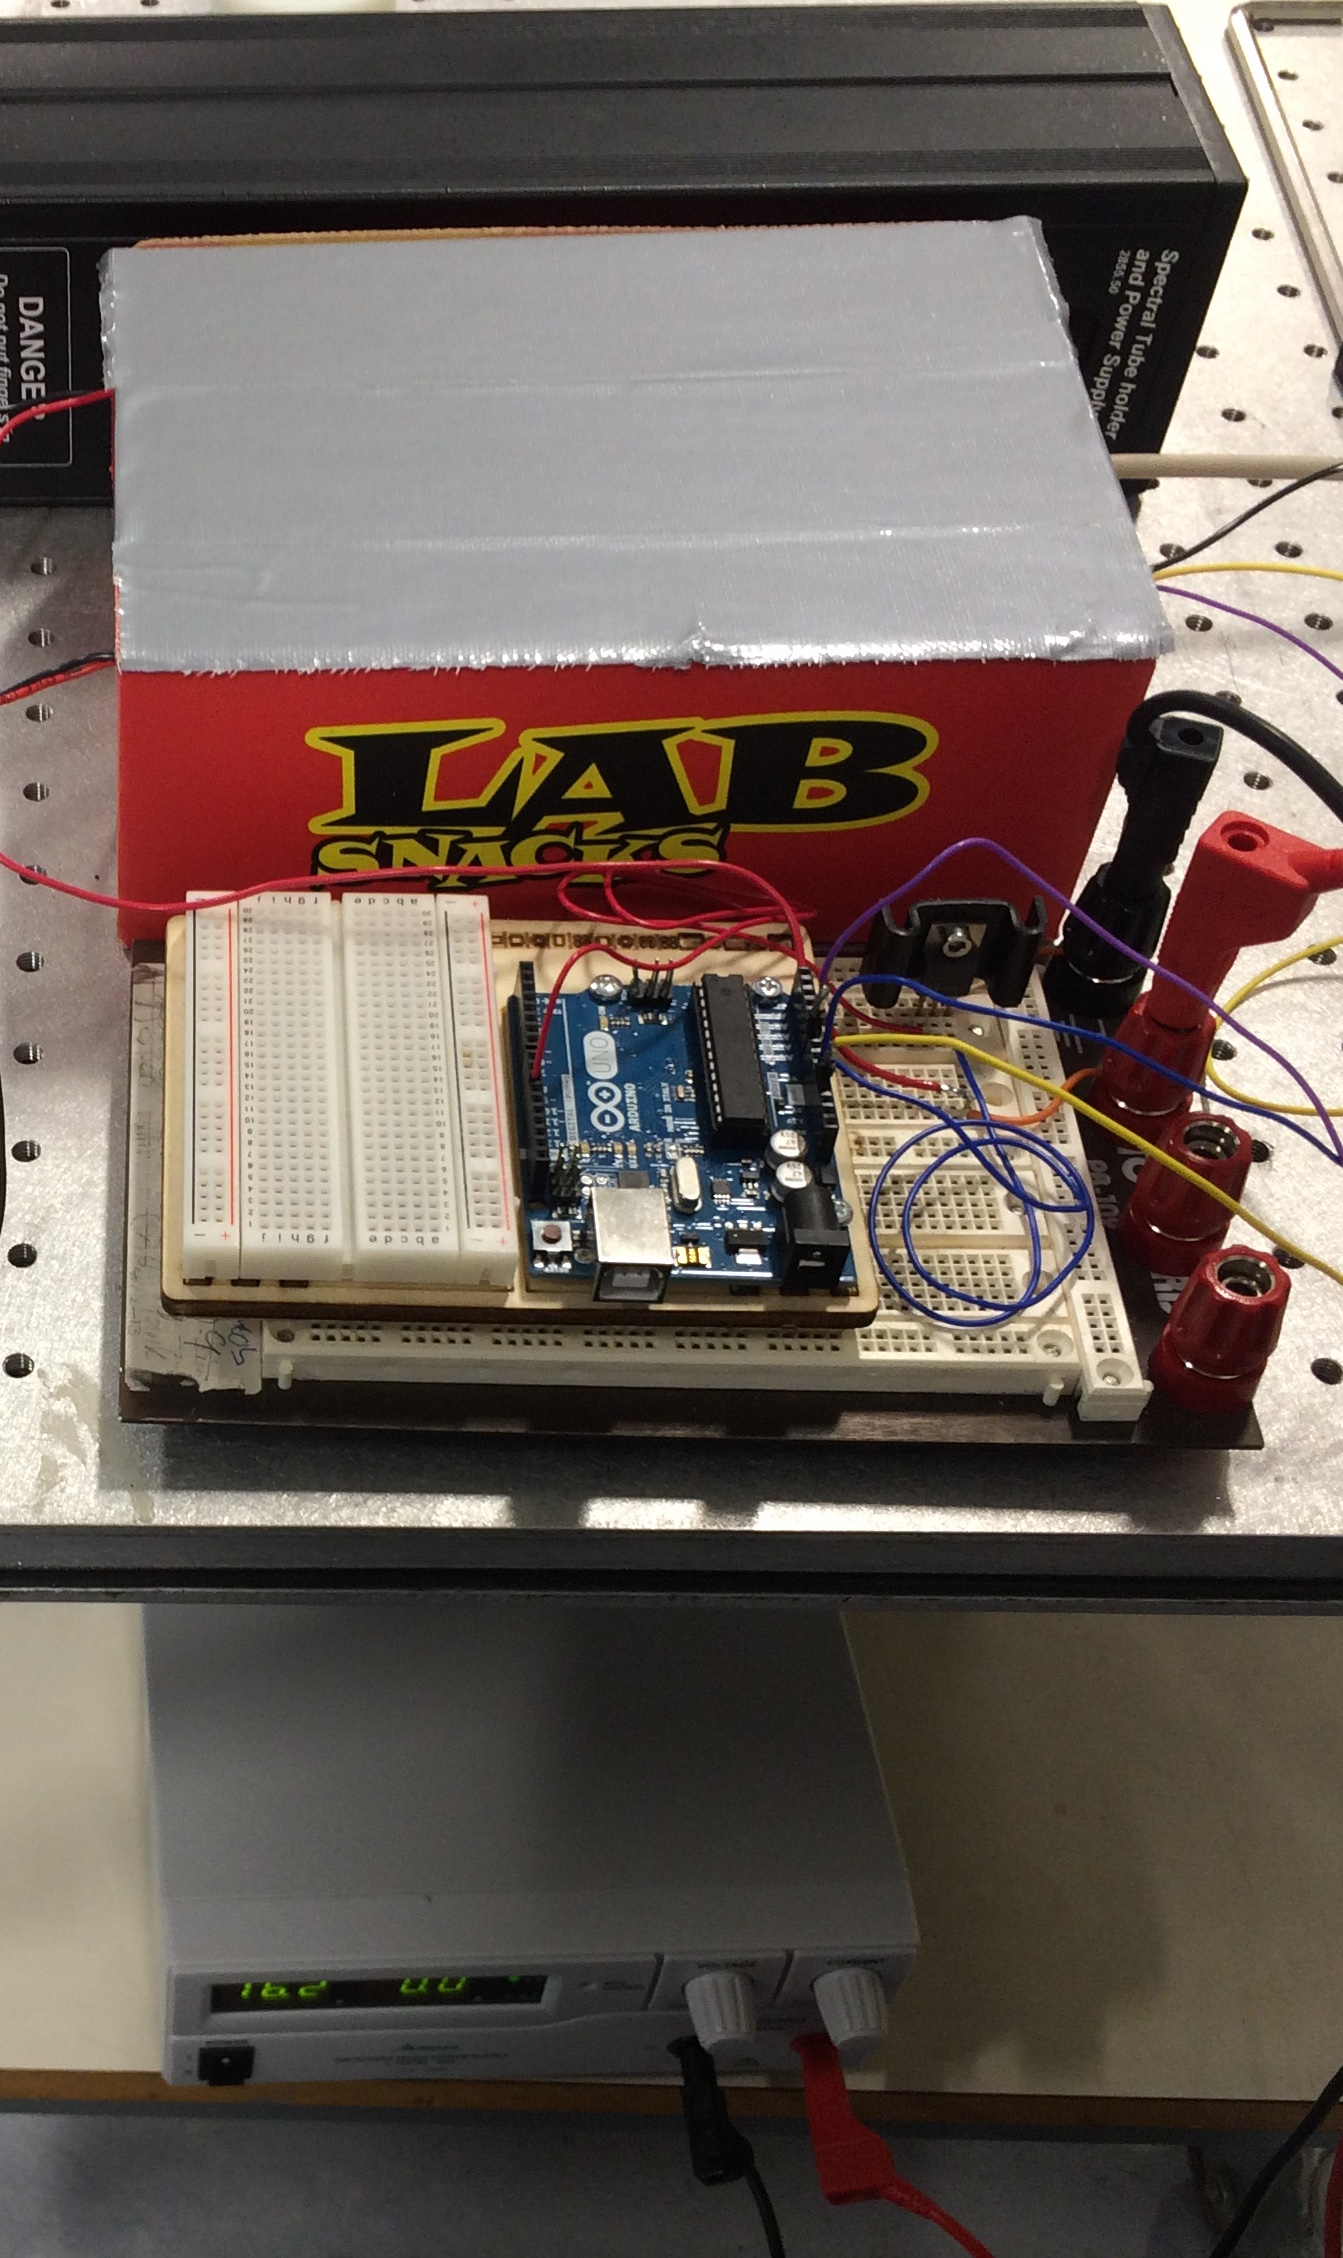
\includegraphics[width=.9\linewidth]{outer_circuit.JPG}
\caption{Outside view of the circuit test.}
\label{fig: outer_circuit}
\end{subfigure}
\caption{The inside and outside view of the setup to test the heater circuit and PID controller. The left panel shows the resistor with heatsink  and the temperature sensor mounted on top of the spectrograph as well as the fan for circulating the air. In the right panel the outside of the setup is shown, including the Helium lamp in the background, the part of the heater circuit located outside the housing.}
\label{fig: cardboard}
\end{figure}

After conducting the initial test of the heater circuit and PID controller some adjustments were made for the final setup to improve stability of the temperature in the housing,
\begin{itemize}
\item The housing was changed to a Styrofoam box for better insulation allowing the set temperature to be reached faster.
\item The resistor and temperature sensor were moved so they were not in contact with the spectrograph, but instead the heating and temperature measurements were done on the circulating air. This was done because it allowed for a more stable temperature within the housing.
 
\end{itemize}

The final setup for the third experiment with the mentioned improvements is shown in Fig. \ref{fig: temp setup final}.
\\
\\
\begin{figure}[h]
\centering
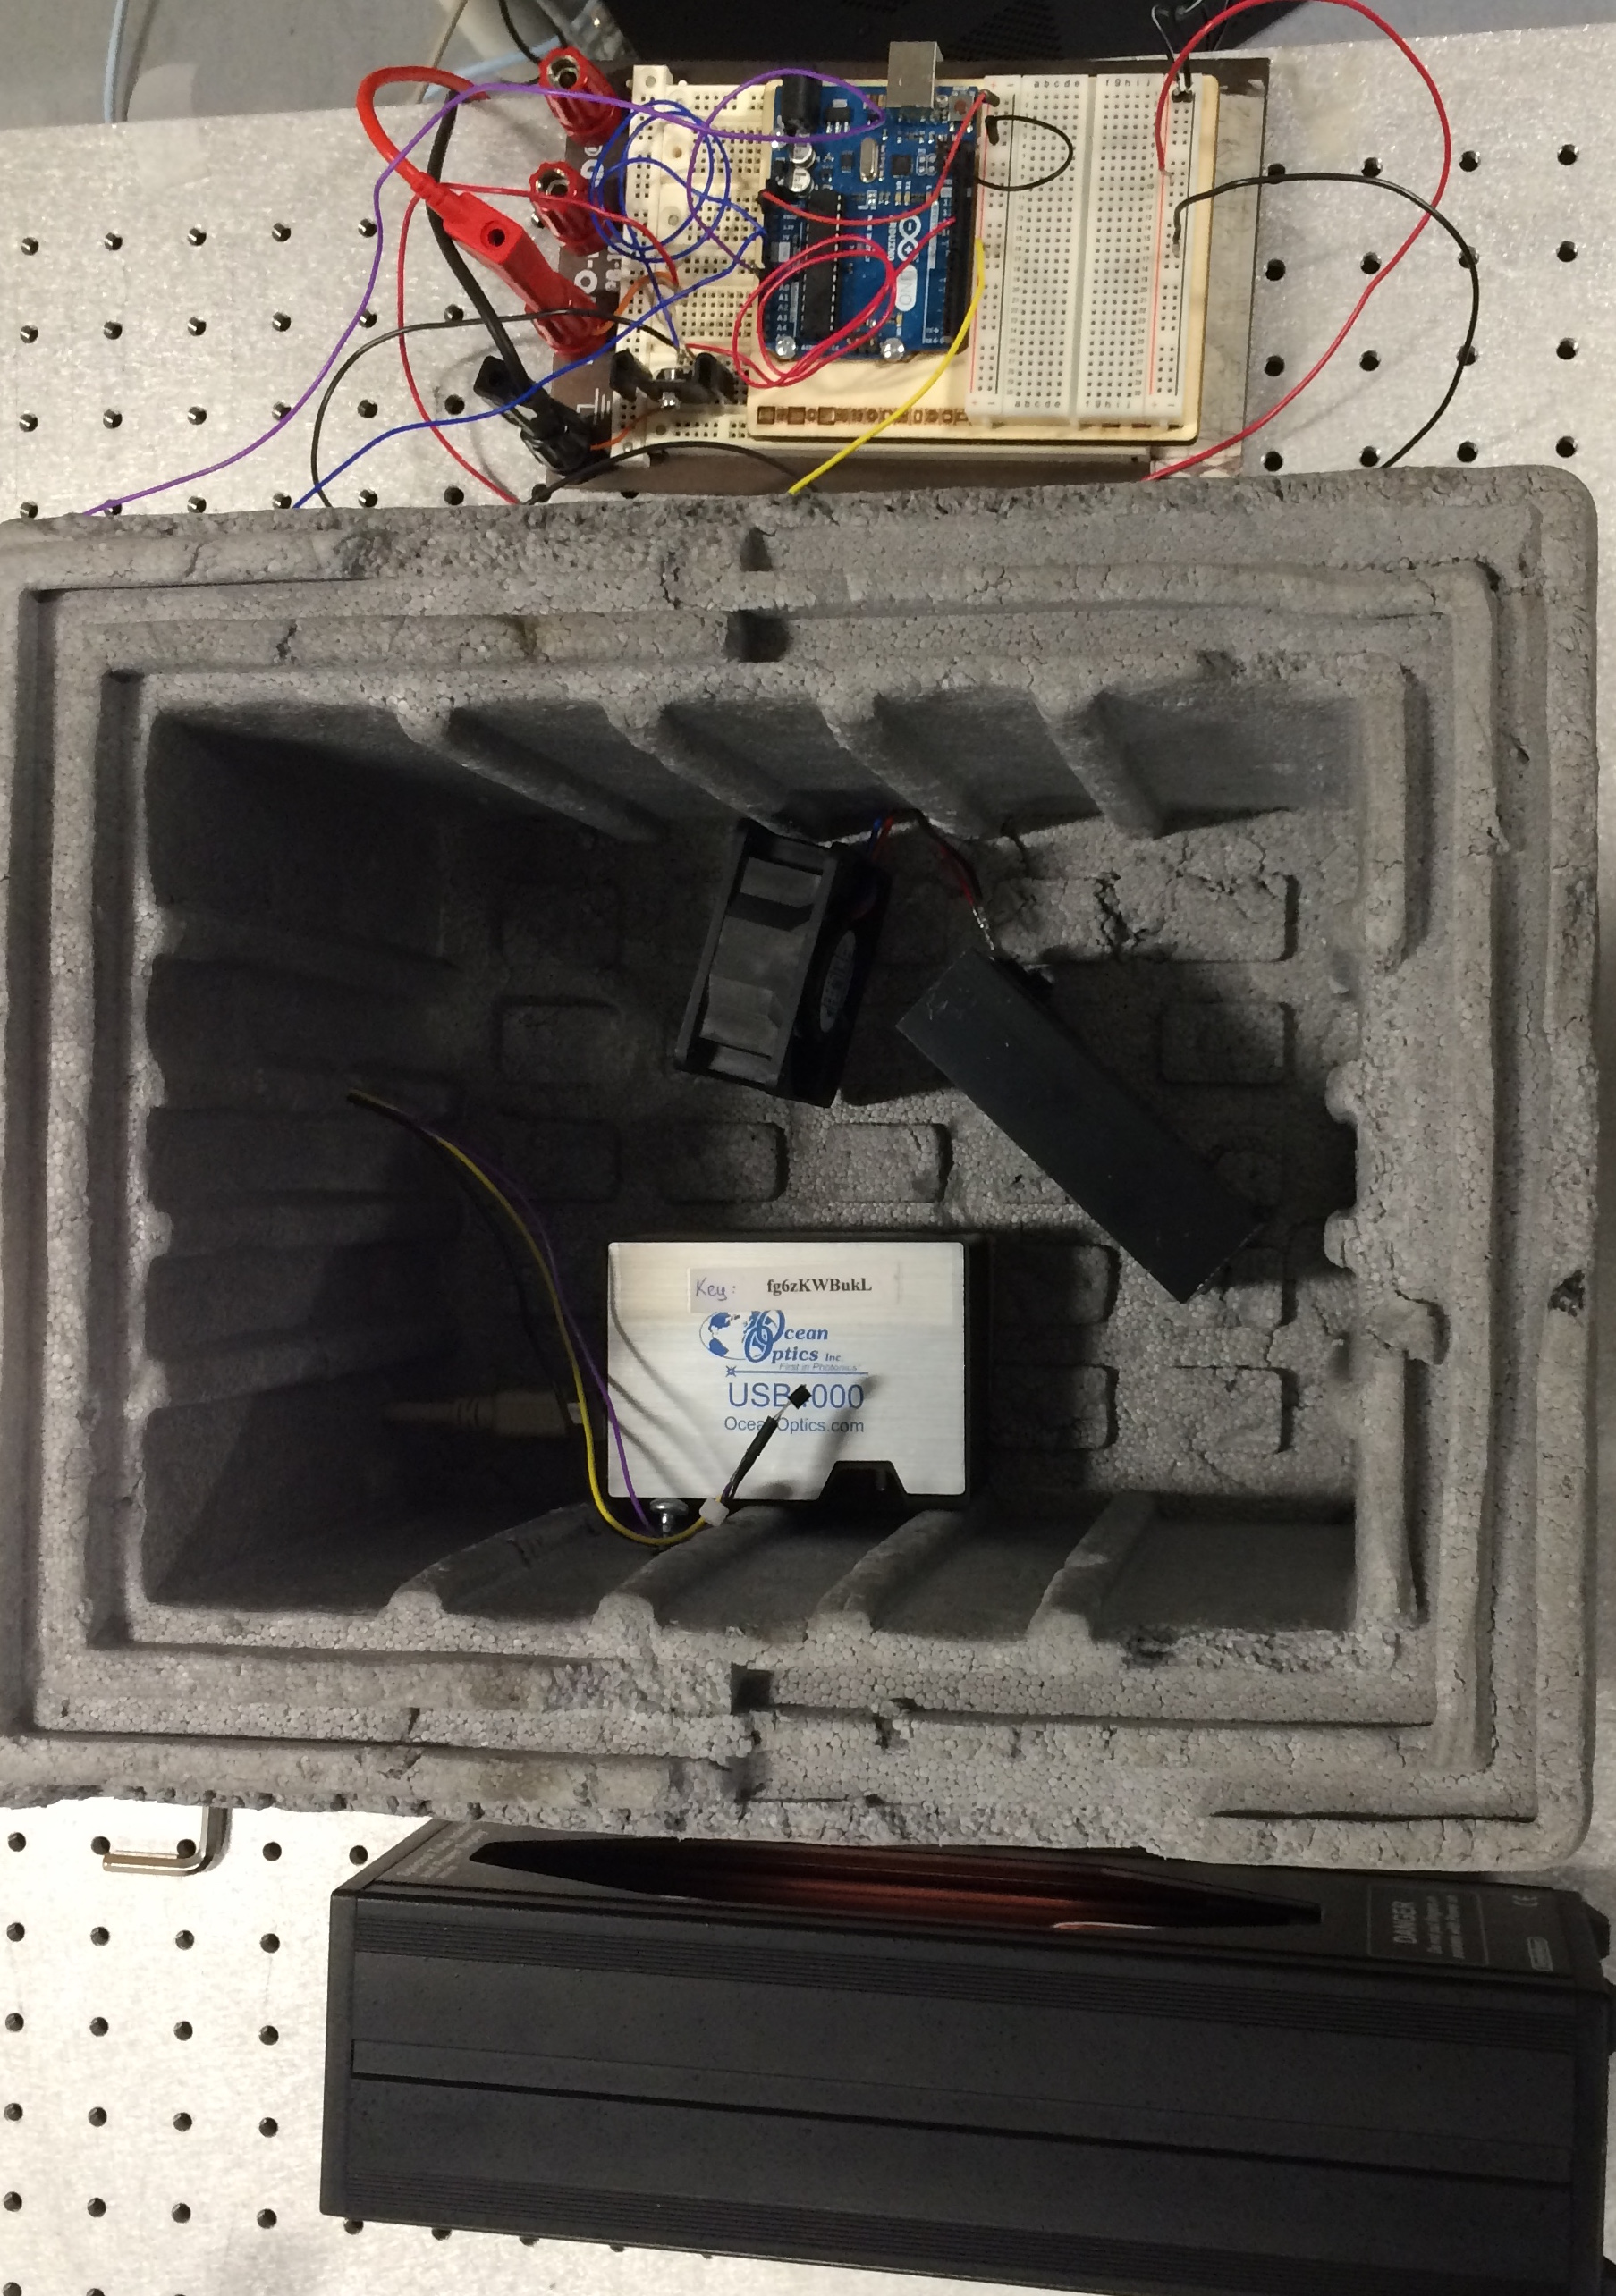
\includegraphics[width=.45\linewidth]{flamingo_circuit.JPG}
\caption{The final setup used for the third experiment. The spectrograph was placed with the entrance slit aligned with the window made in the side of the housing. The resistor with heatsink was placed in front of the fan so the circulating air was heated and the temperature sensor was placed so it measured the air temperature. The housing was closed of with a lid when the experiment was run.}
\label{fig: temp setup final}
\end{figure}

With the final setup decided upon the third experiment was run with the parameters,
\begin{itemize}
\item Measurements were made with the temperature varying from \SI{19.5}{\degreeCelsius} to \SI{49.3}{\degreeCelsius} in eleven steps. Because the spectrograph was heated by the circulating air, the temperature was hold steady for each step for two hours to allow for uniform temperature in the spectrograph.
\item Integration time in \emph{SpectraSuite} was set to \SI{100}{\milli\second} and measurements were taken every \SI{1}{\second} for a total of \num{60} measurements for every temperature step. The intensity of every wavelength was saved to a text file for data processing. 
\end{itemize}





